% \chapter{Fundamentação Teórica}\label{Cap:Fundamentação Teórica}

Neste capítulo serão expostos conceitos necessários para a compreensão desta dissertação. Iniciando pelo processo de formação da voz e conceituando formas como as para catalogar as emoções (Seção \ref{sec:vozemoint}). Em seguida, é feita uma exposição de conceitos relativos a Aprendizagem de Máquina (Seção \ref{sec:ml}), Aprendizado Profundo (Seção \ref{sec:dl}), e abordagens (Seção \ref{sec:spvsup}) aplicadas em tarefas que utilizam esse tipo de tecnologia. Por fim, técnicas para aferir a eficiência (Seção \ref{sec:metricas}) de tarefas de Aprendizagem de Máquina.\\

% ==========================================================================================
\section{Intensidade da Emocão na Voz}\label{sec:vozemoint}

A voz humana é produzida na laringe. Com a passagem do ar oriundo dos pulmões pelas pregas vocais, estas vibram e geram um som. Com o auxílio de outras estruturas fisiológicas como língua, boca e lábios, esse som é transformado e nossa voz é produzida~\cite{51}. Nossa fala não é somente um ato de expressão de ideias e emoções por meio da vocalização~\cite{6.31}, como também é um componente indispensável para a comunicação entre os indivíduos de uma sociedade. Enquanto humanos, somos especialistas em voz, e conseguimos extrair uma gama de informações socialmente relevantes~\cite{49} dessas ondas sonoras.

Nas emoções, temos três modelos bastante consolidados na literatura: Ekman, Russel, e Plutchik. O modelo de Ekman~\cite{31.9} afirma existirem seis emoções básicas: Neutra, raiva, medo, surpresa, alegria e tristeza. E que estas são reconhecidas independentemente do idioma, da cultura ou dos meio de expressão (\textit{i.e.}: fala, expressões faciais, etc.). O modelo de Russel~\cite{31.10} (Figura \ref{fig:russel}), que sugere que as emoções podem ser representadas em um espaço bidimensional, onde o eixo horizontal representa a valência (positiva ou negativa) e o eixo vertical representa a ativação (alta ou baixa). Já o modelo de Plutchik~\cite{57} (Figura \ref{fig:plutchik}), que combina os dois modelos anteriores, criando emoções internas (básicas ou primárias) e externas (compostas ou secundárias).

Plutchik estendeu~\cite{57} o modelo de Russel. Seu modelo, em formato de cone, dispõe de oito emoções básicas com cores distintas. Neste modelo, a intensidade da emoção fica denotada pela intensidade da cor naquela região, indo do mais intenso (centro) para o menos intenso (borda), por exemplo: Com relação ao medo, o terror é mais intenso que a apreensão. As emoções estão dispostas de acordo com seu grau de similaridade: As mais similares estão próximas e as mais antagônicas estão diametralmente opostas. No modelo de Plutchick, as emoções compostas, são aquelas formadas por duas emoções básicas.

A intensidade da emoção pode afetar nossa percepção da mesma~\cite{18.46}. Por exemplo: Felicidade pode ser confundida com euforia, que são semelhantes em qualidade de voz mas distintas quanto a intensidade~\cite{18.9}. Correlacionar a intensidade da emoção com o volume da voz é demasiada simplificação. A intensidade da emoção não pode ser inferida apenas pela energia na fala~\cite{18.12}. As diferenças entre características acústicas da voz podem ser maiores entre diferentes intensidades de uma mesma emoção do que entre emoções diferentes~\cite{18.46}. 

Em~\cite{emoint1}, vemos que indivíduos que experimentam emoções positivas intensas também tendem a experimentar emoções negativas intensas. Bem como a questão de que a intensidade emocional deve ser vista como uma combinação de traço de extroversão e traço de neuroticismo. O reconhecimento de uma função integradora da intensidade da experiência emocional coloca dificuldades do ponto de vista da medida e da metodologia~\cite{emoint2}.

Numa tentativa de resumir a natureza múltipla da intensidade emocional global,~\cite{emoint2.1} nos diz que um dos aspectos mais perceptíveis de uma emoção é a sua intensidade. Quando alguém descreve uma experiência emocional, esta pessoa quase sempre se referirá à sua intensidade. Portanto, é intrigante que esse aspecto da emoção tenha sido quase completamente ignorado como um objeto específico de pesquisa. Também propuseram a seguinte fórmula descritiva: $I_E = f(C, E, A_p, A, P, R)$ onde: $I_E$ denota a intensidade emocional sentida, $C$ a importância dos objetivos ou interesses envolvidos, $E$ a magnitude do acontecimento, $A_p$ uma componente de avaliação, $A$ o potencial de ação, $P$ componentes relevantes de personalidade, e $R$ uma componente de contenção, inibição ou regulação.

Temos~\cite{emoint3}, uma publicação com experimento realizado no Brasil, que busca construir um instrumento de estudo de avaliação psicométrica para mensurar afetos positivos e negativos e confronta seu experimento com outros testes de avaliação de afetos, como a Escala de Afetos Positivos e Negativos (\acrlong{PANAS}, \acrshort{PANAS}) que também foi observada e validade para fins psicométricos, no Brasil, em~\cite{panas1} e~\cite{panas2}. Do ponto de vista do comportamento social,~\cite{16} diz que uma representação da ativação e da intensidade do estado emocional parecem essenciais, mesmo quando a valência não pode ser determinada.


\begin{figure}[!ht]
\centering
\includegraphics[width=0.7\textwidth]{img/modeloderussel.png}
\caption{\label{fig:russel}Modelo de Russel~\cite{img_russel}}
\end{figure}

\begin{figure}[!h]
\centering
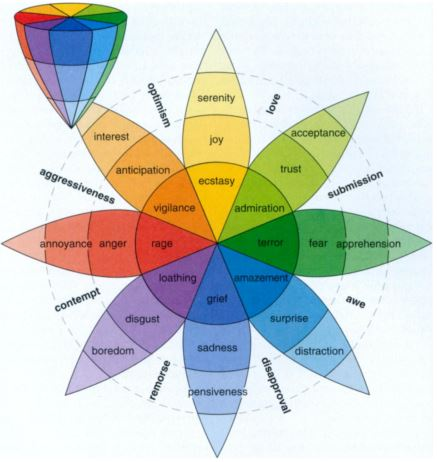
\includegraphics[width=0.6\textwidth]{img/plutchik.JPG}
\caption{\label{fig:plutchik}Modelo de Plutchik~\cite{57}}
\end{figure}

% ==========================================================================================
\section{Aprendizagem de Máquina}\label{sec:ml}

Aprendizagem de Máquina é uma subárea da Inteligência Artificial (\acrlong{AI}, \acrshort{AI}). Inteligência Artificial foi o nome estabelecido~\cite{12.23} para uma área denominada Inteligência Computacional, que consiste no estudo agentes inteligentes. Um agente é algo capaz de atuar num ambiente, enquanto um agente inteligente é um agente que atua no ambiente de forma inteligente, se apropriando de circunstâncias para alcançar um objetivo, possivelmente influenciando o ambiente, com capacidade para alterar esse objetivo, aprendendo com sua experiência e fazendo escolhas adequadas de acordo com suas limitações.

Tarefas de \acrshort{ML} costumam ser descritas em termos de como o sistema de Aprendizagem de Máquina deve processar um exemplo~\cite{53}. Um exemplo consiste numa coleção de recursos, de um objeto ou evento, que foram aferidos quantitativamente e que desejamos que seja processado por esse sistema. Costuma-se representar um exemplo como um vetor $x \in R^n$, onde cada coordenada $x_i$ do vetor $x$ é uma característica (\textit{feature}) desse vetor. Por exemplo, se $x$ representar uma imagem, cada $x_i$ pode ser o valor de um pixel dessa imagem.

Dentre as tarefas de \acrshort{ML}, duas tarefas comuns são a classificação e a regressão. A classificação busca descobrir a qual de $k$ classes possíveis um vetor $x$ pertence, produzindo uma função $f: R^n \rightarrow \{1, ..., k\}$, de modo que quando $y = f(x)$, o modelo atribui a uma entrada (\textit{input}) $x$ uma saída (\textit{output}) numérica de valor $y$ que representa uma categoria (classe). Na regressão, o pensamento é análogo, porém, ao final, o modelo não tenta encontrar a qual classe $x$ pertence, e sim predizer um valor (contínuo) para $f(x)$.

Dentre os algoritmos de \acrshort{ML} utilizados em trabalhos de \acrshort{SER}~\cite{20.7}, encontramos: Floresta Aleatória (\acrlong{RF}, \acrshort{RF}) em~\cite{20.10}, Árvore de Decisão (\acrlong{DT}, \acrshort{DT})~\cite{20.11}, Máquinas de Vetores de Suporte (\acrlong{SVM}, \acrshort{SVM})~\cite{20.13} e K-vizinhos mais próximos (\acrlong{KNN}, \acrshort{KNN})~\cite{20.15}.

% ==========================================================================================
\section{Aprendizado Profundo}\label{sec:dl}

Aprendizado Profundo é um tipo específico de Aprendizado de Máquina~\cite{53}. Algoritmos de \acrshort{ML} citados no parágrafo anterior - conhecidos como algoritmos tradicionais - costumam funcionar bem em uma grande variedade de problemas importantes. Entretanto, não costumam ter desempenho tão bom em problemas que envolvem reconhecimento de fala ou de objetos. O desenvolvimento do Aprendizado Profundo foi motivado, em parte, pela falha desses algoritmos tradicionais em generalizar bem para essas tarefas de Inteligência Artificial.

Dada essa necessidade de explorar modelos mais robustos, alguns trabalhos estudaram o impacto de algoritmos de \acrlong{DL} no reconhecimento de emoção na voz~\cite{12.12, 12.16}.

\begin{figure}[!h]
\centering
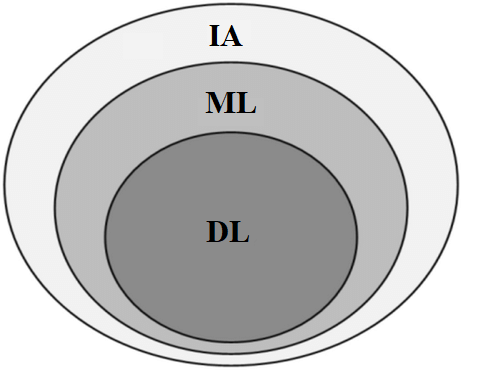
\includegraphics[width=0.4\textwidth]{img/ia-ml-dl-3.png}
\caption{\label{fig:ia-ml-dl}Relação entre \acrshort{IA}, \acrshort{ML} e \acrshort{DL}~\cite{img_iavsmlvsdl}}
\author{Fonte: Retirada de~\cite{58}}
\end{figure}

Redes Multicamadas de Perceptrons (\acrlong{MLP}, \acrshort{MLP}) são predecessoras da construção de modelos de \acrshort{DL}, conhecidos como Redes Neurais (\acrlong{NN}, \acrshort{NN}). O Perceptron é uma unidade (Figura \ref{fig:perceptron}) composta por valores (pesos) $wi$ e uma função de ativação $f$,  que recebe as \textit{fetures}, realiza uma operação matemática entre $wi,xi$, aplica a função de ativação $y = f(x,w)$ e emite esse resultado como \textit{output}.

Podemos realizar o mapeamento de vários Perceptrons, recebendo as \textit{features} e produzindo \textit{outputs}, ao longo de camadas, onde cada camada atua como \textit{input} para a próxima camada, e assim sucessivamente, até chegar a
 um \textit{output} final, assim, temos uma \acrshort{MLP} (Figura \ref{fig:mlp}).
 
 % (Figura\footnote{Imagem adaptada, gerada em \url{http://alexlenail.me/NN-SVG/index.html}}\ref{fig:mlp}).
 
 A camada inicial é chamada de camada de entrada (\textit{input layer}), as camadas intermediárias são chamadas de camadas ocultas (\textit{hidden layers}) e a camada final é chamada de camada de saída (\textit{output layer}). Compreendendo uma rede neural como um conjunto de nós e arestas, cada nó da rede será chamado de neurônio.

\begin{figure}[!ht]
\centering
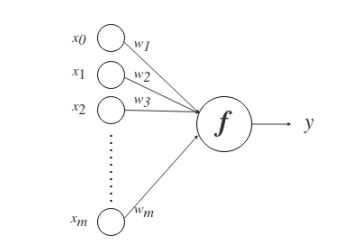
\includegraphics[width=0.6\textwidth]{img/perceptron.png}
\caption{\label{fig:perceptron}Exemplo de Perceptron}
\author{Fonte: Retirado de~\cite{12}}
\end{figure}

\begin{figure}[!h]
\centering
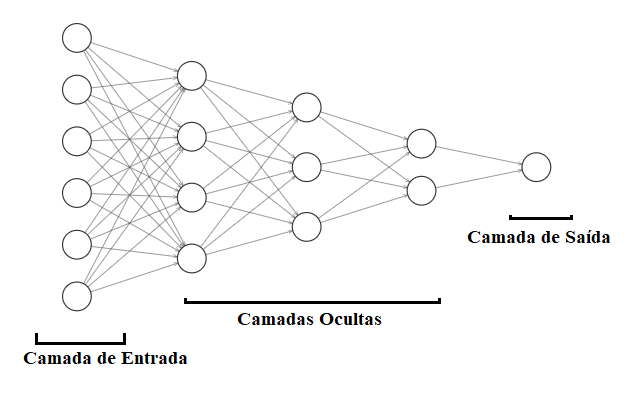
\includegraphics[width=0.6\textwidth]{img/mlp03.png}
\caption{\label{fig:mlp}Exemplo de arquitetura \acrshort{MLP}}

\end{figure}

% ------------------------------------------------------------------------------------------
\subsection{Redes Neurais Profundas}

Nosso cérebro tem uma grande capacidade de generalização, o que nos ajuda a raciocinar de forma indutiva e é o primeiro passo do nosso aprendizado~\cite{32}. Redes neurais são capazes de aprender relações não lienares complexas e criar relações entre \textit{input} e \textit{output}, formando sistemas utilizados em várias áreas de \acrshort{ML}, e \acrshort{SER} não é uma exceção~\cite{32.74}.

Com base no conceito e organização de uma rede neural, o conjunto formado pela disposição dos neurônios, pesos e funções de ativação pode ser organizado de forma a criar diferentes arquiteturas que ao longo do tempo se mostraram eficientes para generalizar bem em certas áreas de conhecimento. Diremos que uma rede neural se torna uma Rede Neural Profunda quando possui grande quantidade de neurônios e camadas ocultas em sua arquitetura, embora não haja um valor específico que a habilite a se tornar profunda ao superá-lo.

% \footnote{Exemplos visuais de diversas arquiteturas de DL: \url{https://www.asimovinstitute.org/neural-network-zoo/}}

% \footnote{Gerada em \url{http://alexlenail.me/NN-SVG/index.html}} 

% \begin{figure}[!h]
% \centering
% 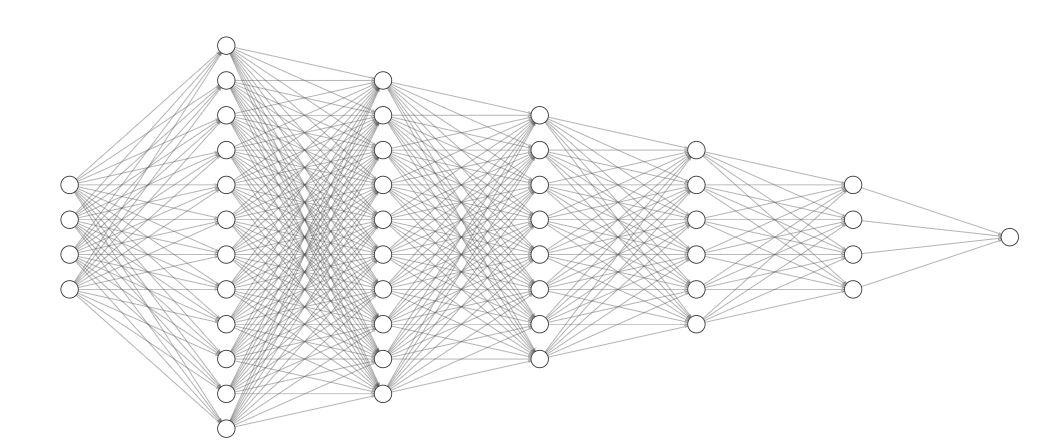
\includegraphics[width=0.6\textwidth]{img/ex-dnn.JPG}
% \caption{\label{fig:exarqdnn}Exemplo de arquitetura \acrlong{DNN}}
% \end{figure}

A seguir, abordaremos duas dessas arquiteturas que se mostram importantes para este trabalho: Redes Neurais Convolucionais e Autoencoder.


% ==========================================================================================
\section{Abordagens Supervisionada e Não Supervisionada}\label{sec:spvsup}

No processo de criação de modelos de \acrshort{ML}, uma vez definida a arquitetura, a rede irá começar a aprender com os dados de forma iterativa. A etapa onde o modelo começa a ver os \textit{inputs} e tentar inferir a classe é chamada de treinamento (\textit{training}). Duas abordagens tradicionais para esse momento são a Aprendizagem Supervisionada (\textit{Supervised Learning}) e a Aprendizagem Não Supervisionada (\textit{Unsupervised Learning}).

% ------------------------------------------------------------------------------------------
\subsection{Abordagem Supervisionada}

Para a primeira, é necessário que os dados já estejam rotulados com a classe (\textit{label}) a qual cada registro de pertence. Por exemplo, ao utilizar uma base de dados que envolve imagens, pode ser trivial etiquetar os dados com base no objeto que aparece naquela imagem (\textit{e.g.}: ou gato ou cachorro). Para emoções essa atividade irá demandar pessoas especializadas e capacitadas. Uma pesquisa~\cite{32} recente (2021) aponta essa dificuldade na área de \acrshort{SER}, pois mesmo quando há variedade de conjuntos de dados (\textit{datasets}) diferentes, estes podem apresentar poucas classes, poucos registros por classe ou ambos.

Sejam $X, Y$, conjuntos de \textit{inputs} e \textit{outputs}, respectivamente, $X=\{x_i, ..., x_n\}$ e $Y=\{y_i, ..., y_n\}$, onde o $y_i$ é a classe de $x_i$, podemos generalizar a etapa de treinamento como seguinte fluxo $\forall x_i \in X' \subset X$:

Seja $f: X \rightarrow Y,$ tal que $f(x) = y$, então,

\begin{enumerate}
    \item O modelo $f$ é apresentado a um dado $x_i$ e produz um resultado $f(x_i) = y_i'$;
    \item É calculado um erro $d_i = d(y_i, y_i')$ entre o resultado apresentado e o resultado esperado;
    \item $d_i$ É utilizado para atualizar os parâmetros de $f$;
    \item O processo é repetido para o próximo exemplo $x_{i+1}$.
\end{enumerate}

A etapa de treinamento costuma ser seguida pela etapa de testes (\textit{tests}), onde o modelo é exposto aos $x_j \in (X \setminus X')$ e, a partir daí, são calculadas métricas para aferir o desempenho de $f$.

Cabe observar que $f$ não precisa ser injetora, uma vez que mais de um $x_i$ pode pertencer a mesma classe $y_i$.

\subsection{Abordagem Não Supervisionada}

Para uma abordagem não supervisionada, os modelos são apresentados a um conjunto de dados sem rótulos e tentam aprender características importantes da sua estrutura. A distinção entre supervisionado e não supervisionado costuma se dar pela presença ou não da classe (\textit{target}) daqueles dados. Note que é possível aplicar uma abordagem não supervisionada a um \textit{dataset} mesmo quando a classe é conhecida, basta excluí-la do processo de treinamento do modelo.

Alguns casos de uso de \textit{Unsupervised Learning} incluem: (1) Formação de conjuntos (\textit{clustering}); (2) \textit{Feature Learning}; (3) Redução de dimensionalidade; (4) Automatizar a rotulação de amostras; (5) Aprender sobre o \textit{dataset} através de análise exploratória (\acrlong{EDA}, \acrshort{EDA}).

Trabalhos envolvendo aprendizado não supervisionado apontam as capacidades de Autocodificadores (\acrlong{AE}, \acrshort{AE}) tanto para aprendizagem de características\textit{feature learning}~\cite{35.16, 35.17} quanto para redução de dimensionalidade~\cite{35.18, 35.19}.


% ==========================================================================================
\section{Métricas de Avaliação de Modelos}\label{sec:metricas}

Modelos de aprendizagem de máquina precisam ser validados para que possamos avaliar o seu desempenho e gerar inferências a respeito do seu comportamento. Existem diversas formas, para avaliar seus resultados, sendo esta mais ou menos adequadas à natureza do modelo. Na lista abaixo temos variáveis utilizadas para calcular métricas de avaliação do treinamento e teste de modelos de \acrshort{ML}:

\begin{itemize}
    \item Verdadeiros Positivos (VP) ou \acrlong{TP} (\acrshort{TP}): Classificação correta da classes positivas;
    \item Verdadeiros Negativos (VN) ou \acrlong{TN} (\acrshort{TN}): Classificação correta da classes negativas;
    \item Falsos Positivos (FP) ou \acrlong{FP} (\acrshort{FP}): Erro onde o modelo previu uma classe positiva, quando o valor real pertencia a classe negativa;
    \item Falsos Negativos (FN) ou \acrlong{FN} (\acrshort{FN}): Erro onde o modelo previu uma classe negativa, quando o valor real pertencia a classe positiva.
\end{itemize}

Com essas variáveis, podemos calcular as seguintes métricas:

\begin{itemize}
    \item Acurácia (\textit{Accuracy}): Indica a performance geral do modelo.
        \begin{equation}
        \frac{VP + VN}{VP+FP+FN+FN}
        \end{equation}
    \item Precisão (\textit{Precision}): Dentre as classificações positivas que o modelo fez, quais foram corretas.
        \begin{equation}
        \frac{VP}{VP+FP}
        \end{equation}
    \item Sensibilidade (\textit{Recall}): Dentre todas as classificações positivas esperadas, quantas foram corretas.
        \begin{equation}
        \frac{VP}{VP+FN}
        \end{equation}
    \item \textit{F1-Score}: Média harmônica entre precisão e sensibilidade.
        \begin{equation}
        2 * \frac{precision  * recall}{precision + recall}
        \end{equation}
\end{itemize}

% ==========================================================================================
\section{Considerações Parciais}

Neste capítulo, foram abordados os principais conceitos para fornecer subsídios a esta Dissertação. Em razão disso, foi dada uma maior ênfase no que tange os dados a serem utilizados, insumo deste trabalho. A partir dos conceitos apresentados, foram citados trabalhos relacionados que os utilizam, demonstrando a aderência desse trabalho as práticas utilizadas nesta área de pesquisa. Mais detalhes da estratégia deste trabalho, como aquisição dos dados e arquitetura dos e detalhes dos modelos serão apresentados Capítulo 4. No capítulo a seguir, serão apresentados trabalhos relacionados a este com o intuito de identificar e validar as lacunas deste tema na literatura. 
